\chapter{Implementation}\label{chapter:implementation}

% \section{Device drivers in Linux}
% In the Linux operating system, device drivers play a pivotal role in the management and operation of hardware. They serve as the interface between the hardware and the software, allowing the operating system and applications that run on it to interact with hardware components without needing to understand the details of how the hardware operates. This abstraction is vital for the development of a stable, portable, and scalable operating system.

% Linux drivers interact with the kernel and hardware through a set of predefined kernel functions. This interface abstracts away the complexities of the hardware and provides a consistent programming interface for driver developers. A driver typically registers itself with the kernel to handle specific hardware device IDs, and the kernel then calls into the driver when the application or system requires operations on this device. The operations a driver can perform include initialisation, reading data from or writing data to the device, and handling interrupts triggered by the hardware.

% \subsection{Kernel space}
% One of the fundamental concepts in Linux and Unix-like operating systems is the division between user space and kernel space. This division is crucial for system security and stability.

% Being a monolithic kernel, Linux's operating system runs entirely in kernel space, meaning it has complete access to the hardware and can execute any CPU instruction and access any memory address. Kernel space is highly protected because faults here can cause the entire system to crash. Device drivers primarily operate in kernel space, allowing them to directly control hardware and execute privileged operations necessary for their tasks. For user space applications, Linux offers multiple APIs to access block devices, these being the standard file I/O API \texttt{read()}/\texttt{write()}, \texttt{libaio}, and \texttt{io\_uring}, the latter two enabling asynchronous read and write operations to block devices.

\section{User space drivers}
Like SPDK, our driver runs entirely in user space, and implements zero-copy I/O operations, as well as a poll-based architecture; SPDK\footnote{\url{https://spdk.io}} being the de-facto standard for NVMe devices in high throughput environments. To write a user space driver, we make use of all the concepts explained in \autoref{chapter:basics}. The driver is able to access the device after memory mapping device files from user space, which offers more flexibility, simplicity, and stability over kernel drivers, with access to debugging tools and overall less restrictions the development of user space drivers is much easier and the ability to use any programming language is also guaranteed. User space drivers are also less likely to cause system crashes or kernel panics due to bugs; faults in user space can often be handled gracefully, improving overall system stability. By avoiding context switches, these drivers are able to reduce overall latency and throughput.

Given these advantages, we chose to develop a user space NVMe driver rather than kernel space.

\section{Memory-Mapped I/O}\label{section:MMIO}

In our code, mapping the BARs to main memory is done by the function \texttt{pci\_map\_resource()} (see \autoref{lst:mmap}) in \texttt{pci.rs}. Here, we open the \texttt{resource0} file with read and write access and pass the file descriptor and its length to \texttt{libc::map}. As \texttt{libc::mmap} directly calls \texttt{mmap(2)}, the function call is wrapped in an \texttt{unsafe} block. If the function returns a null pointer or the length of the file is 0, we return an error, otherwise the pointer and the length of the file are returned as a pair.

\begin{lstlisting}[float, language=Rust,label=lst:mmap,caption=Memory mapping a PCI resource in Rust]
pub fn pci_map_resource(pci_addr: &str) -> Result<(*mut u8, usize), Error> {
    let path = format!("sys/bus/pci/devices/{}/resource0", pci_addr);

    let file = fs::OpenOptions::new().read(true).write(true).open(&path)?;
    let len = fs::metadata(&path)?.len() as usize;

    let ptr = unsafe {
        libc::mmap(
            ptr::null_mut(),
            len,
            libc::PROT_READ | libc::PROT_WRITE,
            libc::MAP_SHARED,
            file.as_raw_fd(),
            0,
        ) as *mut u8
    };

    if ptr.is_null() || len == 0 {
        Err("pci mapping failed".into())
    } else {
        Ok((ptr, len))
    }
}
\end{lstlisting}

\section{Direct Memory Access}
To enable the transfer of data between the host system and NVMe device we make use of DMA. We initialise DMA memory for all Submission and Completion Queues, as well as buffers where the device can read from and write to.
Enabling the usage of huge pages on the operating system is done with the shell script \texttt{setup-hugetlbfs.sh} which creates a mount point for huge pages and writes a number of huge pages to \texttt{sysfs} files. Now we can allocate memory by creating the file in the newly mounted directory and then memory map the file with \texttt{mmap(2)} and lock it in memory with \texttt{mlock(2)} by using the appropriate bindings in the \texttt{libc} crate. We then derive the physical memory address of the page through \texttt{/proc/self/pagemap}.

\begin{figure}
  \centering
    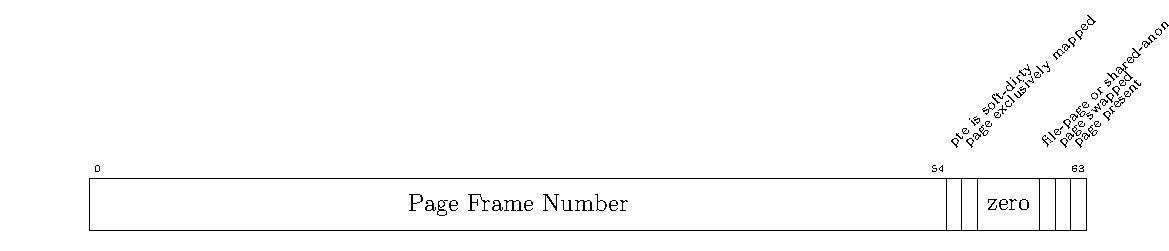
\includegraphics[width=\textwidth]{figures/pagemap}
    \caption{Fields of a pagemap entry when the page is present in main memory}
    \label{fig:pagemap}
\end{figure}

The pagemap contains one 64 bit value for each virtual page; our hugepage is in main memory, so the pagemap entry is structured as depicted \autoref{fig:pagemap}. Finding the relative index of the page is done by taking the virtual address of it and dividing it by the the page size, which we use to locate the corresponding pagemap entry. Constructing the physical address from the pagemap entry and virtual address is done by taking the Page Frame Number (Bits 0-54), multiplying that by the page size to get the physical address of the page frame, to which we add (virtual address$\mod$page size), the offset within the page frame. \autoref{lst:virt_phys} shows how this is done in Rust.

One of the reasons the driver runs as root is due to requiring \texttt{CAP\_SYS\_ADMIN} to be able to read the Page Frame Numbers since the Rowhammer vulnerability exploit, i.e. since Linux 4.0.

\begin{lstlisting}[float, language=Rust, label=lst:virt_phys,caption=Translating a virtual address to its physical address]
fn virt_to_phys(addr: usize) -> Result<usize, Error> {
    let pagesize = unsafe { libc::sysconf(libc::_SC_PAGESIZE) } as usize;

    let mut file = fs::OpenOptions::new()
        .read(true)
        .open("/proc/self/pagemap")?;

    file.seek(io::SeekFrom::Start(
        (addr / pagesize * mem::size_of::<usize>()) as u64,
    ))?;

    let mut buffer = [0_u8; mem::size_of::<usize>()];
    file.read_exact(&mut buffer)?;

    let phys = unsafe {
      mem::transmute::<[u8; mem::size_of::<usize>()], usize>(buffer)
    };
    Ok((phys & 0x007F_FFFF_FFFF_FFFF) * pagesize + addr % pagesize)
}
\end{lstlisting}

In \texttt{memory.rs} we define the struct \texttt{Dma<T>} with the method \texttt{allocate()}, which allocates a huge page and maps it to memory, and returns a struct encapsulating a virtual address to the object of type \texttt{T} and the physical address. We also define the trait \texttt{DmaSlice} with the functions \texttt{chunks()} and \texttt{slice()}, which we use for zero-copy I/O operations.

% \section{Architecture}

\section{Driver initialisation}
In this section, we will go over the initialisation process of the driver, looking what happens within the function \texttt{init()} in \texttt{lib.rs} and the functions it calls; \texttt{init()} returns an instance of \texttt{NvmeDevice}, if nothing goes wrong. The struct is the driver for a single NVMe drive, and can handle admin and I/O requests.

Before any configuration and initialisation is done, we check if the PCI device has the class id \texttt{0x0108}: \texttt{0x01} for mass storage device, \texttt{0x08} the NVMe subclass.
We then unbind the kernel driver from the NVMe device by writing the PCI address of the device to the \texttt{unbind} file in \texttt{sysfs}. This is then followed by enabling the bus master and disabling interrupts by setting the appropriate bits in the PCI command register, thus enabling DMA and disabling interrupts entirely, as our driver is poll-based. At this point, we also initialise all the relevant structs required for the driver e.g., admin and I/O queues.

The BARs of the NVMe device is then mapped into main memory, as described in \autoref{section:MMIO}. We then follow the initialisation procedure described in the NVMe specification: first, we disable the controller by setting the \texttt{EN} (enable) bit to 0 in the \texttt{CC} (Controller Configuration) register. We wait for the \texttt{ready} bit in the \texttt{CSTS} register to be set to 0, after which we can configure the controller. Then, we set the \texttt{ASQ} (Admin Submission Queue), \texttt{ACQ} (Admin Completion Queue) and the \texttt{AQA} (Admin Queue Attributes) to the physical addresses of the queues and the queue length, respectively. This is followed by setting the submission and completion entry sizes in \texttt{CC}. The controller is then enabled by setting the \texttt{EN} bit to 1, and we wait for the \texttt{CSTS} register to be set to 1. Now the NVMe controller is ready to process admin submissions. The relevant offsets for the registers are stored in the enum \texttt{NvmeRegs32} and \texttt{NvmeRegs64}.

Although we use unsafe functions to access the BARs of the NVMe device, with an assertion guard, we can make sure that all accesses to the registers are not out of bound (see \autoref{lst:reg32}).

% accessing register be like
\begin{lstlisting}[float, language=Rust, label=lst:reg32,caption=Writing to a 32-bit register]
fn set_reg32(&self, reg: u32, value: u32) {
    assert!(reg as usize <= self.len - 4, "memory access out of bounds");
    unsafe {
      std::ptr::write_volatile(
        (self.addr as usize + reg as usize) as *mut u32, value
      );
    }
}
\end{lstlisting}

After this, we request an I/O completion queue, followed by a request for an I/O submission queue, so the \texttt{NvmeDevice} can do I/O operations. Then we identify the namespaces, which get stored in a \texttt{HashMap} in the \texttt{NvmeDevice}.

\section{I/O operations}\label{subsection:io}
As all commands are processed through submission and completion queues, we have defined the structs \texttt{NvmeSubQueue}, and \texttt{NvmeCompQueue}, which store a \texttt{NvmeCommand} array, and \texttt{NvmeCompletion} array on a huge page, respectively. The submission entry being 64 bytes in size means that at most 1024 entries fit on a 2 MiB huge page; for simplicity, we have not implemented queues which span over multiple pages. Thus the maximum number of outstanding submissions we currently support is 1023.

The struct \texttt{NvmeDevice} is able to run as the driver itself, handling admin and I/O commands and also polling their completions, thus it exposes I/O operations with the methods \texttt{read()}, \texttt{write()},  \texttt{read\_copied()}, \texttt{write\_copied()}, as well as \texttt{read\_batched()} and \texttt{write\_batched()}. The initial two methods are zero-copy, taking a reference to a struct which implements the trait \texttt{DmaSlice} as the source buffer for writes and destination for reads, allowing us to iterate over the object in 8096 byte chunks. Currently we only iterate over 8096 bytes, as that is the maximum length we can pass to the NVMe command without the use of PRP lists. If we were to use PRP lists, each request would require constructing a PRP list on a DMA-able buffer.

The latter four methods take a \texttt{u8} slice, which gets copied into the \texttt{NvmeDevice}'s DMA buffer for writes, and copied from for reads. In \texttt{read\_copied()} and \texttt{write\_copied()} we iterate over 512 KiB chunks, which is equal to 128 PRP list entries, as for some reason the I/O operation returns an error when the list is longer than 128 entries. \texttt{read\_batched()} and \texttt{write\_batched()} both take a parameter specifying the batch size of the operation. Here we also iterate over 512 KiB chunks, but instead of a single submission request for each chunk, we split it into multiple submissions which get simultaneously added to the queue and polled for. As NVMe SSDs can process multiple submissions at once, batching generally leads to higher throughput, similarly to how increasing queue depth improves performance.

Similar to SPDK, \texttt{NvmeDevice} can also create a submission and completion queue pair \texttt{NvmeQueuePair} with the method \texttt{create\_io\_queue\_pair()}. We enable multithreading by allowing each thread to have their own queue pair, submitting I/O requests with \texttt{submit\_io()}, which like \texttt{read()} and \texttt{write()} receives a reference to a \texttt{impl DmaSlice}. This method iterates over 8096 KiB as well and returns the number of requests added to the submission queue. It is the user's responsibility to poll for the completion of a command with \texttt{complete\_io()}, which takes the number of submissions to poll for and returns an \texttt{Option<NvmeCompletion>}.

Aside from the data buffer, the user also passed the logical block address (LBA) for the I/O operation. The length of data written is derived from the length of the buffer.
